\section{Introduction}
\begin{frame}{Instability of Plasma Flow}
  \begin{itemize}
    \item The instability of plasma flow refers to the tendency of a plasma system to deviate from a stable, equilibrium state and exhibit perturbations or fluctuations in its behavior. \cite{chen_introduction_2016}
  \end{itemize}  
  To investigate instability, we assume oscillating perturbed quantities , $\tilde{n}, \tilde{v} \sim \exp(-i\omega t)$.
  \begin{enumerate}
    \item If $\Im(\omega) > 0$, then it is unstable flow since the perturbations grow exponential in time, $\exp(\Im(\omega) t)$. 
    \item If $\Im(\omega) <=0$, then it is stable flow since the perturbations decay/unchanged in time.
  \end{enumerate}
\end{frame}

\begin{frame}{Magnetic Nozzle}
  \begin{itemize}
    \item A magnetic nozzle is a device that uses a magnetic field to shape and control the flow of charged particles in a plasma propulsion system.
    \item Instabilities may affect magnetic nozzle operation and the resulting thrust. \cite{kaganovich_2020_physics}
  \end{itemize}
  \begin{figure}[htbp]
    \centering
    \begin{subfigure}{0.45\textwidth}
      \centering
      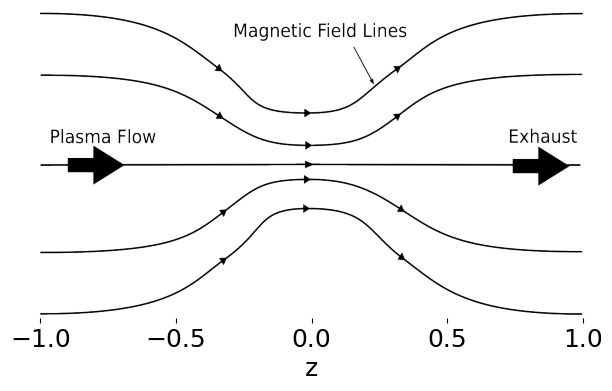
\includegraphics[width=0.8\linewidth]{figures/magnetic-nozzle}
      \caption{Simplified representation of magnetic nozzle.} 
    \end{subfigure}%
    \begin{subfigure}{0.45\textwidth}
      \centering
      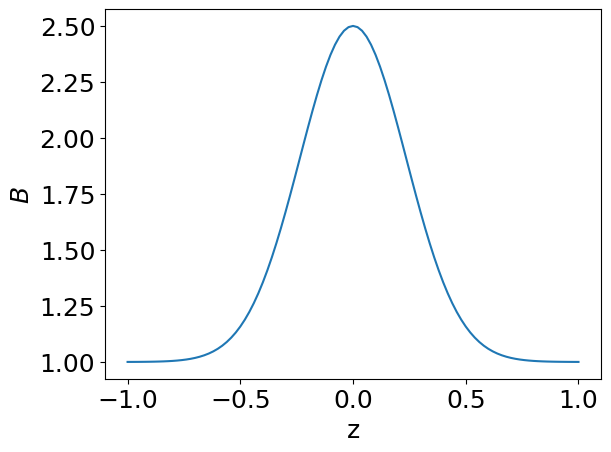
\includegraphics[width=0.8\linewidth]{figures/magnetic-field}
      \caption{A simplified magnetic field of magnetic nozzle.} 
    \end{subfigure}
    \caption{Simplified representation of magnetic nozzle. Length is normalized.}
    \label{fig:magnetic-nozzle}
  \end{figure}
\end{frame}

\begin{frame}{Governing Equations}
  The nondimensionalized governing equations for the plasma flow in magnetic nozzle are 
  \begin{align}
    & \text{Cons. of Den.}  &&\pdv{n}{t} + n\pdv{v}{z} + v\pdv{n}{z} - nv\frac{\partial_z B}{B} = 0 \\
    & \text{Cons. of Mom.}  &&n\pdv{v}{t} + nv\pdv{v}{z} = -\pdv{n}{z}
  \end{align}
  where $n,v$ are density and velocity, respectively. 

  The equilibrium quantities $n_0, v_0$ must satify the condition, 
  \begin{align}
      &\pdv{z}(\frac{n_0v_0}{B}) = 0 \label{eq:equilibrium-convervation-of-mass}\\
      &v_0\pdv{v_0}{z} = -\frac{1}{n_0}\pdv{n_0}{z} \label{eq:equilibrium-convervation-of-momentum}
  \end{align}
\end{frame}
 
\begin{frame}{Polynomial Eigenvalue Problem}
  By linearizing the governing equations, and assume oscillating perturbed quantities, $\tilde{n}, \tilde{v} \sim \exp(-i\omega t)$. We can derive the following equation,

  \begin{equation}
    \begin{aligned}
      &\omega^2 \tilde{v} \\ 
      +& 2i\omega\left(v_0\pdv{}{z} + \pdv{v_0}{z}\right) \tilde{v} \\
      +& \left[ (1-v_0^2)\pdv[2]{}{z} 
        -\left(3v_0 + \frac{1}{v_0}\right)\pdv{v_0}{z}\pdv{}{z} \right. \\
        &- \left. \left(1-\frac{1}{v_0^2}\right)\left(\pdv{v_0}{z}\right)^2 
      - \left(v_0+\frac{1}{v_0}\right)\pdv[2]{v_0}{z} \right]\tilde{v}
      = 0
    \end{aligned}
    \label{eq:polynomial_eigenvalue_problem}
  \end{equation}

  It is a polynomial eigenvalue problem.
\end{frame}
